\documentclass{article}


\usepackage[utf8]{inputenc}
\usepackage[a4paper, total={6in, 9in}]{geometry}
\usepackage{braket}
\usepackage{xcolor}
\usepackage{amsmath}
\usepackage{amsfonts}
\usepackage{tikz}
\usepackage{svg}
\usepackage{graphicx}
\usepackage{media9}
\usepackage{float}
\usetikzlibrary{calc}
\usepackage{array}
\usepackage[ruled,vlined,linesnumbered]{algorithm2e}

\usepackage[
backend=biber,
style=alphabetic,
sorting=ynt
]{biblatex}



\newcommand{\commentt}[1]{\textcolor{blue}{ \textbf{[COMMENT]} #1}}
\newcommand{\ctt}[1]{\commentt{#1}}
\newcommand{\prb}[1]{ \mathbf{Pr} \left[ {#1} \right]}
\newcommand{\onotation}[1]{\(\mathcal{O} \left( {#1}  \right) \)}
\newcommand{\ona}[1]{\onotation{#1}}
\newcommand{\nvar}[2]{ \( #1_{1}, #1_{2} ... #1_{#2}  \) }
%\newenvironment{proof}[0]{\paragraph{Proof.}}{}
%\newenvironment{remark}[0]{\textit{remark}}{}
\newenvironment{cor}[0]{\paragraph{Corollary.}}{}
\newenvironment{example}[0]{\paragraph{Example.}}{}
%\newenvironment{thm}[0]{\paragraph{Theorem.}}{}
\newtheorem{prop}{Proposition}
\newtheorem{ex}{Exercise}
\newtheorem{sol}{Solution}
\newtheorem{theorem}{Theorem} 		
\newtheorem{thm}{Theorem}[section]
\newtheorem{conj}[thm]{Conjecture} 	
\newtheorem{lemma}[thm]{Lemma}
\newtheorem{corollary}[thm]{Corollary} 
\newtheorem{claim}[thm]{Claim}
\newtheorem{proposition}[thm]{Proposition}
\newtheorem{definition}{Definition} 
\newtheorem{remark}{Remark}
 


% \addbibresource{sample.bib} %Import the bibliography file
\begin{document}    
\maketitle
\begin{document}
\setcounter{chapter}{2}
\chapter{Recursive Analysis - Recitation} 
%\author{Master theorem and recursive trees.}
% 
%\begin{abstract}
%    One of the standard methods to analyze the running time of algorithms is to express recursively the number of operations that are made. In the following recitation, we will review the techniques to handle such formulation (solve or bound).  
%\end{abstract}
%

\section{Bounding recursive functions by hands.} Our primary tool to handle recursive relation is the Master Theorem, which was proved in the lecture. As we would like to have a more solid grasp, let's return on the calculation in the proof over a specific case. 
Assume that your algorithm analysis has brought the following recursive relation:
    \begin{example}\( T\left(n\right)  = \left\{ \begin{array}{rcl}
& 4T\left(\frac{n}{2}\right)+c\cdot n & \mbox{for }  n > 1  \\
& 1 & \mbox{else}  
\end{array}\right. \). Thus, the running time is given by \begin{equation*}
    \begin{split}
 & T\left(n\right)  = 4T\left(\frac{n}{2}\right)+c\cdot n=  4\cdot4T\left(\frac{n}{4}\right)+4c\cdot\frac{n}{2}+c\cdot n = ... = \\ & \overset{\text{\textcolor{red}{critical}}}{\overbrace{4^{h}T(1)}} + c\cdot n\left(1+\frac{4}{2}+\left(\frac{4}{2}\right)^{2}...+\left(\frac{4}{2}\right)^{h-1}\right) = 4^{h} + c\cdot n\cdot\frac{2^{h}-1}{2-1}
    \end{split}
\end{equation*}
We will call the number of iteration till the stopping condition the recursion height, and we will denote it by \(h\) . What should be the recursion height? \( 2^{h} = n \Rightarrow h =\log\left(n\right) \). So in total we get that the algorithm running time equals \( \Theta\left(n^2\right)\). 
\end{example}
\textbf{Question}, Why is the term \( 4^{h} T(1) \) so critical? Consider the case \(T\left(n\right) =  4T\left(\frac{n}{2}\right) + c \) .One popular mistake is to forget the final term, which yields a linear solution \( \Theta(n)\) (instead of quadric \( \Theta(n^2)\)).   

    \begin{example}\( T\left(n\right)  = \left\{ \begin{array}{rcl}
& 3T\left(\frac{n}{2}\right) + c\cdot n & \mbox{for }  n > 1  \\
& 1 & \mbox{else}  
\end{array}\right. \), and then the expanding yields: 
\begin{equation*}
    \begin{split}
        T\left(n\right) & = 3T\left(\frac{n}{2}\right) + c\cdot n = 3^2 T\left(\frac{n}{2^2}\right) + \frac{3}{2}cn + c\cdot n =  \overset{\text{\textcolor{red}{critical}}}{\overbrace{3^{h}T(1)}} + cn\left(1 + \frac{3}{2} + \left(\frac{3}{2}\right)^2 + ...  + \left(\frac{3}{2}\right)^{h-1} \right) \\
        & h = \log_{2}\left(n\right) \Rightarrow T\left(n\right) = 3^{h}T(1) + c\cdot \textcolor{red}{n}\cdot \left(\left(\frac{3}{\textcolor{red}{2}}\right)^{\log_{2}{n}}\right) / \left(\frac{3}{2} - 1\right) = \theta \left( 3^{\log_{2}(n)} \right) =  \theta \left( n^{\log 3} \right)  
    \end{split}
\end{equation*}
where \(n^{\log 3}  \sim n^{1.58} < n^2 \).
\end{example}


\section{Master Theorem, one Theorem to bound them all. }
As you might already notice, the same pattern has been used to bound both algorithms. The master theorem is the result of the recursive expansion. it classifies recursive functions at the form of \(T\left(n\right) = a\cdot T\left( \frac{n}{b} \right) + f\left(n\right) \), for positive function \(f : \mathbb{N} \rightarrow \mathbb{R}^{+} \).       

\begin{defbox}{Master Theorem, simple version.} First, Consider the case that \(f = n^c\). Let \( a \ge 1, b > 1\) and \( c \ge 0 \). then: 
\begin{enumerate}
    \item if \(\frac{a}{b^c} < 1 \) then \( T\left(n\right) = \Theta \left( n^c \right) \) \ \ \ \textbf{(\(f\) wins)}.
    \item if \(\frac{a}{b^c} = 1 \) then \( T\left(n\right) = \Theta \left( n^c \log_{b} \left(n\right) \right) \).
    \item if \(\frac{a}{b^c} > 1 \) then \( T\left(n\right) = \Theta \left( n^{\log_{b} \left(a\right)} \right) \) \ \ \ \textbf{(\(f\) loose)}.
  \end{enumerate}
\end{defbox}

\begin{example}  \( T\left(n\right)  =4T\left(\frac{n}{2}\right)+d\cdot n \Rightarrow
T\left(n\right) = \Theta\left(n^2\right)\) according to case (3). And \(T\left(n\right)  = 3T\left(\frac{n}{2}\right) + d\cdot n \Rightarrow T\left(n\right) = \Theta \left( n^{\log_{2}\left(3\right)}\right)\)
also due to case (3).
\end{example}
\begin{defbox}{Master Theorem, strong version.} 
Now, let's generalize the simple version for arbitrary positive \(f\) and let~\(a~\ge~1~,~b~>~1\). 

\newcommand{\logab}{\log_{b} \left(a\right)}

\begin{enumerate}
    \item if  \(f\left(n\right) = O \left( n^{\logab - \varepsilon }\right)\) for some \( \varepsilon > 0 \) then \( T\left(n\right) = \theta \left( n^{\logab} \right) \) \ \ \ \textbf{(\(f\) loose)}.
    
    \item if  \(f\left(n\right) = \Theta \left( n^{\logab} \right) \) then \( T\left(n\right) = \Theta \left( n^{\logab}  \log\left(n\right)\right) \)
    
    \item if there exist \(\varepsilon >0 ,c<1\) and \(n_0 \in \mathbb{N} \) such that  \(f\left(n\right) = \Omega \left( n^{\logab + \varepsilon }\right)\) and for every \( n > n_0 \) \(a \cdot f\left( \frac{n}{b} \right) \le c f\left(n\right)\)  then \( T\left(n\right) = \theta \left( f\left(n\right) \right) \) \ \ \ \textbf{(\(f\) wins)}.
    
\end{enumerate}
\end{defbox}
\newcommand{\TT}[2]{#1 T\left(\frac{n}{#2}\right)}

\begin{example} 
\begin{enumerate}
    \item \( T\left(n\right) =  T\left(\frac{2n}{3}\right) + 1 \rightarrow f\left(n\right) = 1 =\Theta \left( n^{\log_{\frac{3}{2}} \left(1\right)}\right)\) matches the second case. i.e  \( T\left(n\right) = \Theta \left( n^{\log_{\frac{3}{2}} \left(1\right)}\log n \right)\).
    
    \item \( T\left(n\right) = \TT{3}{4} + n\log n \rightarrow f\left(n\right) = \Omega\left( n^{\log_{4}\left(3\right) + \varepsilon}  \right) \) and notice that \( f\left( a\frac{n}{b}\right) = \frac{3n}{4}\log\left(\frac{3n}{4}\right)\) . Thus, it's matching to the third case. \(\Rightarrow T\left(n\right) = \Theta\left(n\log n\right)\).
    
    \item \(T\left(n\right) = 3T\left( n^{\frac{1}{3}}\right) + \log\log n\). let \( m = \log n \Rightarrow T\left( n\right) = T \left(2^m \right) = 3T\left(2^{\frac{m}{3}} \right) + \log m\). denote by \(S = S\left(m\right) = T\left(2^m\right) \rightarrow S\left(m\right) = 3T\left(2^{\frac{m}{3}} \right) + \log m = 3S\left(\frac{m}{3} \right) + \log m\). And by the fact that \(\log m = O\left(m^{\log_{3}\left(3\right)-\varepsilon} \right) \rightarrow T\left(n\right) = T\left(2^m\right) = S\left(m\right) = \Theta\left(m\right) = \Theta\left( \log(n)\right) \).  
\end{enumerate}
\end{example}

\section{Recursive trees.}
There are still cases which aren't treated by the \textit{Master Theorem}. For example consider the function \(T\left(n\right) = 2T\left(\frac{n}{2}\right) + n\log n \). Note, that \(f = \Omega\left( n^{\log_{b}(a)} \right) = \Omega\left(n\right)\). Yet for every \( \varepsilon > 0 \Rightarrow f = n\log n = O\left( n^{1+\varepsilon} \right) \) therefore the third case  doesn't hold. How can such cases still be analyzed? 

\paragraph{Recursive trees Recipe}
    \begin{enumerate}
        \item draw the computation tree, and calculate it's height. in our case, \( h = \log n \).
        \item calculate the work which done over node at the \(k\)-th level, and the number of nodes in each level. in our case, there are \(2^k\) nodes and over each we perform \(f(n) = \frac{n}{2^k} \log\left( \frac{n}{2^k}\right)\) operations. 
        \item sum up the work of the \(k\)-th level.
        \item finally, the total time is the summation over all the \( k \in [h]\) levels. 
    \end{enumerate}
applying the above, yields 
\begin{equation*} 
\begin{split} 
T\left(n\right) & =  \sum_{k=1}^{\log{n}}{n\cdot\log \left( \frac{n}{2^k}\right)} = n\sum_{k=1}^{\log{n}}{ \left( \log n - \log 2^k \right) } 
  = n\sum_{k=1}^{\log{n}}{ \left( \log n - k \right) } = \\ & = \Theta \left( n \log^2 \left(n\right)  \right) 
\end{split}
\end{equation*}

\begin{example}
Consider merge sort variation such that instead of splitting the array into two equals parts it's split them into different size arrays. The first one contains \( \frac{n}{10} \) elements while second contains the others \( \frac{9n}{10}\) elements.

%\begin{algbox}{non-equal-merge alg.}
\begin{algorithm}
\SetAlgoLined
\KwResult{returns the sorted permutation of \(x_1 ... x_n \in \mathbb{R}^n \)  }
 \ \\ 
 \If{ \(n \le 10 \) }
    { return bubble-sort \( (x_1 ... x_n)\) } 
 \ \\ 
 
 \Else {
 define \(S_{l} \leftarrow x_1 ... x_{\frac{n}{10}-2}, x_{\frac{n}{10}-1} \) \\
 define \(S_{r} \leftarrow   x_{\frac{n}{10}},x_{\frac{n}{10}+1} ...,x_n \) \\
 \ \\ 
 \( R_l \leftarrow \) non-equal-merge\( \left( S_l \right) \) \\ 
 \( R_r \leftarrow \) non-equal-merge\( \left( S_r \right) \) \\
 \ \\
 return Merge(\(R_l, R_r\))
  
 }
\end{algorithm}
%\end{algbox}
Note, that the master theorem achieves an upper bound, 
\begin{equation*}
    \begin{split}
        T\left(n\right) & = n +  T\left(\frac{n}{10}\right) + T\left(\frac{9n}{10}\right) \le n +  2 T\left(\frac{9n}{10}\right) \Rightarrow T\left(n\right) = O \left( n^{\log_{\frac{10}{9}}\left(2\right)} \right) \sim O \left( n^{ 6 } \right)  
    \end{split}
\end{equation*}
Yet, that bound is far from been tight. Let's try to count the operations for each node. Let's try another direction. 

\begin{claim}
Let \(n_i\) be the size of the subset which is processed at the \(i\)-th node. Then for every \(k\):
\begin{equation*}
    \sum_{i \in \text{k level}}{n_i} \le n
\end{equation*}
\end{claim}
\begin{proof} Assuming otherwise implies that there exist index \(j\) such that \(x_j\) appear in at least two different nodes in the same level, denote them by \(u,v\). As they both are in the same level, non of them can be ancestor of the other. denote by \(m \in \mathbb{N}\) the input size of the sub array which is processed by the the lowest common ancestor of \(u\) and \(v\), and by \(j^\prime \in [m]\) the position of \(x_j\) in that sub array. By the definition of the algorithm it steams that \(j^\prime < \frac{m}{10} \) and \(j^\prime \ge \frac{m}{10}\). contradiction.  The height of the tree is bounded by \( \log_{\frac{9}{10}} \left(n\right) \). Therefore the total work equals \( \Theta \left( n\log n \right) \). Thus, the total running time equals to:
\begin{equation*}
    T(n) = \sum_{k \in \text{levels}}{\sum_{i \in \text{k level}}{f\left(n_i\right)}} = \sum_{k \in \text{levels}}{\sum_{i \in \text{k level}}{n_i}} \le n\log n  
\end{equation*}
\end{proof}
\end{example}

%Please write a tikz code of a computation tree, each node contain an array, the recursive call split the array into two unbalacend parts, the left son will always get a 1/3 of the array while the right get 2/3 of it. please draw at least 3 levels. 
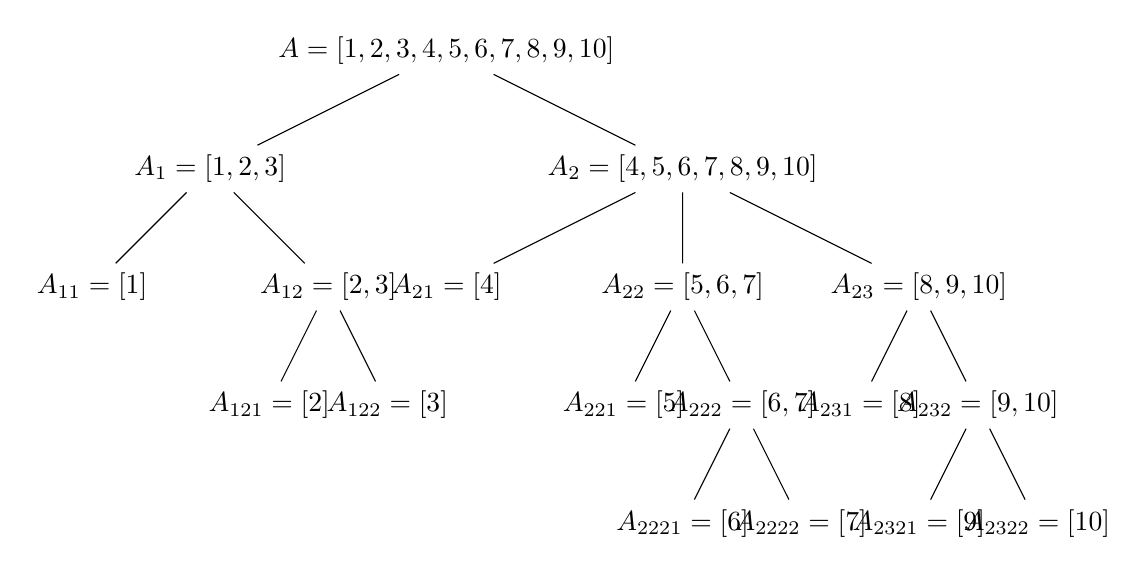
\begin{tikzpicture}[level distance=1.5cm,
  level 1/.style={sibling distance=6cm},
  level 2/.style={sibling distance=3cm},
  level 3/.style={sibling distance=1.5cm}]
  \node (root) {$A=[1,2,3,4,5,6,7,8,9,10]$}
    child {node {$A_1=[1,2,3]$}
      child {node {$A_{11}=[1]$}}
      child {node {$A_{12}=[2,3]$}
        child {node {$A_{121}=[2]$}}
        child {node {$A_{122}=[3]$}}
      }
    }
    child {node {$A_2=[4,5,6,7,8,9,10]$}
      child {node {$A_{21}=[4]$}}
      child {node {$A_{22}=[5,6,7]$}
        child {node {$A_{221}=[5]$}}
        child {node {$A_{222}=[6,7]$}
          child {node {$A_{2221}=[6]$}}
          child {node {$A_{2222}=[7]$}}
        }
      }
      child {node {$A_{23}=[8,9,10]$}
        child {node {$A_{231}=[8]$}}
        child {node {$A_{232}=[9,10]$}
          child {node {$A_{2321}=[9]$}}
          child {node {$A_{2322}=[10]$}}
        }
      }
    };
\end{tikzpicture}


\ifdefined\BOOK


\section{Appendix. Recursive Functions In Computer Science. (Beyond the scope of the 2024 course.)}


%\ctt{The current section repeats over part of the content above as it was designed to be self-contained. Also, notice that this part is considered as optional material and you are not required to remember the following algorithms for the final exam. Its primary goal is to expose you to "strange" running times. }


\begin{example}[Leading Example. numbers multiplication.]
Let \(x,y\) be an \(n\)'th digits numbers over \( \mathbb{F}^{n}_{2} \). It's known that summing such a pair requires a linear number of operations. Write an algorithm that calculates the multiplication \(x\cdot y\). 
\end{example}
\begin{example}[Long multiplication.]
To understand the real power of the dividing and conquer method, let's first examine the known solution from elementary school.  In that technics, we calculate the power order and the value of the digit separately and sum up the results at the end. Formally: \(x \leftarrow \sum_{i=0}^{n}{x_{i}2^{i}}\) Thus, \[ x\cdot y =\left( \sum_{i=0}^{n}{x_{i}2^{i}} \right) \left( \sum_{i=0}^{n}{y_{i}2^{i}} \right) =  \sum_{i,j \in [n]\times[n] }{ x_{i}y_{j}2^{i+j} }\] the above is a sum up over \(n^2\) numbers, each at length \(n\) and therefore the total running time of the algorithm is bounded by \( \theta(n^3) \). \ctt{ notice that adding \(1\) to \(1111111111...1\) requires \(O(n)\) }.
\end{example}
\begin{example}[Recursive Approach.] We could split \(x\) into the pair \(x_{l}, x_{r}\) such that \(x = x_{l} + 2^{\frac{n}{2}}x_{r} \). Then the multiplication of two \(n\)-long numbers will be reduced to sum up over multiplication of a quartet. Each at length \(\frac{n}{2}\). Thus, the running time is given by \begin{equation*}
    \begin{split}
 x\cdot y & = \left(x_{l} + 2^{\frac{n}{2}}x_{r}\right)\left(y_{l} + 2^{\frac{n}{2}}y_{r}\right) = x_{l}y_{l} + 2^{\frac{n}{2}} \left( x_{l}y_{r} + x_{r}y_{l} \right) + 2^{n}x_{r}y_{r} \\ &  \Rightarrow T\left(n\right)  =4T\left(\frac{n}{2}\right)+c\cdot n=4\cdot4T\left(\frac{n}{4}\right)+4c\cdot\frac{n}{2}+c\cdot n = ... = \\ & c\cdot n\left(1+\frac{4}{2}+\left(\frac{4}{2}\right)^{2}...+\left(\frac{4}{2}\right)^{h-1}\right) + 4^{h}T(1) = n^{2} + c\cdot n\cdot\frac{2^{h}-1}{2-1}
    \end{split}
\end{equation*}
We will call the number of iteration till the stopping condition the recursion height, and we will denote it by \(h\) . What should be the recursion height? \( 2^{h} = n \Rightarrow h =\log\left(n\right) \). So in total we get that multiplication could be achieved by performs \( \Theta\left(n^2\right)\) operations. 
\end{example}
\paragraph{Karatsuba algorithm.}
%Many years it was believed that multiplication can't done by less then $\Omega\left(n^2\right)$ time; until Karatsuba found the following algorithm \cite{Karatsuba1963MultiplicationOM}. Let $z_{0},z_{1}z_{3}$ defined as follow: \begin{equation*}
It was once thought that multiplication could not be done in less than $\Omega\left(n^2\right)$ time; however, Karatsuba discovered an algorithm \cite{Karatsuba1963MultiplicationOM} that proved this wrong. Let $z_{0},z_{1}z_{3}$ be defined as follows:
\begin{equation*}
z_0, z_1, z_2 \leftarrow x_{l}y_{r}, x_{l}y_{r} + x_{r}y_{l}, x_{r}y_{r}
\end{equation*}Notice that \( z_1 = \left(x_{l}+x_{r}\right)\left(y_{l}+y_{r}\right) - z_{0} -z_{1} \). summarize the above yields the following pseudo code. 

%\begin{algbox}{Karatsuba alg.}
\begin{algorithm}
\SetAlgoLined
\KwResult{returns the multiplication \(x\cdot y\) where \(x,y \in \mathbb{F}^{n}_{2}\) }
 \ \\ 
 \If{ \(x,y \in \mathbb{F}_{2}\) }
    { return \(x \cdot y\) } 
 \ \\ 
 
 \Else {
 define \(x_{l} , x_{r} \leftarrow x \) and \(y_{l} , y_{r} \leftarrow x \) \ \ \ \ \ // \( O \left(n\right) \). \\ 
 \ \\ 
 calculate \(z_0 \leftarrow \text{Karatsuba}\left(x_{l},y_{l}\right)\) \\
 \ \ \ \ \ \ \ \ \ \ \ \ \(z_2 \leftarrow \text{Karatsuba}\left(x_{r},y_{r}\right)\) \\ 
 \ \ \ \ \ \ \ \ \ \ \ \ \(z_1 \leftarrow \text{Karatsuba}\left(x_{r} + x_{l} ,y_{l} + y_{r} \right) - z_0 - z_2 \) \\ 
 \ \\
 return \(z_0 + 2^{\frac{n}{2}}z_1 + 2^{n}z_2\) \ \ \ \ \  // \( O \left(n\right) \). 
 }
\end{algorithm}
%\end{algbox}
Let's analyze the running time of the algorithm above, assume that \(n = 2^{m}\) and then the recursive relation is 
\begin{equation*}
    \begin{split}
        T\left(n\right) & = 3T\left(\frac{n}{2}\right) + c\cdot n = 3^2 T\left(\frac{n}{2^2}\right) + \frac{3}{2}cn + c\cdot n = cn\left(1 + \frac{3}{2} + \left(\frac{3}{2}\right)^2 + ...  + \left(\frac{3}{2}\right)^{h-1} \right) + ) + 3^{h}T(1) \\
        & h = \log_{2}\left(n\right) \Rightarrow T\left(n\right) = n^{\log_{2}{3}} +  c\cdot \textcolor{red}{n}\cdot \left(\left(\frac{3}{\textcolor{red}{2}}\right)^{\log_{2}{n}}\right) / \left(\frac{3}{2} - 1\right) = \theta \left( 3^{\log_{2}(n)} \right) =  \theta \left( n^{\log 3} \right)  
    \end{split}
\end{equation*}
where \(n^{\log 3}  \sim n^{1.58} < n^2 \).

\fi


% \printbibliography 
\end{document}


